\chapter{Implementation}

\section{TastyTruffle Intermediate Representation}

As Scala programs in \acrshort{tasty} format are unsuitable for execution in a Truffle interpreter, programs in TASTy must be parsed and transformed into an executable intermediate representation in \textsc{TastyTruffle}. The following sections will introduce the nodes in TastyTruffle IR and how they are derived from Scala source and TASTy.

TODO: insert TASTy tree diagrams.

\subsection{Root Node}

\subsection{Read and Write Nodes}

\subsubsection{\mintinline{scala}|(x: )|}

\subsection{Control Flow Nodes}

\subsection{Call Nodes}

\subsection{Type Nodes}

\subsection{Allocation Nodes}

\subsubsection{\mintinline{scala}|new Foo|}

\subsubsection{\mintinline{scala}|new Array[Int]|}

\subsubsection{\mintinline{scala}|new Array[T]|}

\subsection{Example}

\begin{figure}[H]
	\begin{minted}{scala}
		def checksum[T](data: Array[T]): Int = {
			val sum: Int = 0
			var index: Int = 0
			while (index < data.length) {
				val sum += data[i].##
				index += 1
			}
			
			return sum	
		}
	\end{minted}
	\caption{Example implementation of a checksum function.}
\end{figure}

\section{Specialization}

Cover the types of specializable terms.

\section{Specializing Methods}

\subsection{Code Path Duplication}

\subsection{Typed Dispatch}

\subsection{Partial Evaluation}

Use pseudocode example to show partial evaluation? Algorithm? GraalIR?

\begin{figure}
	\centering
	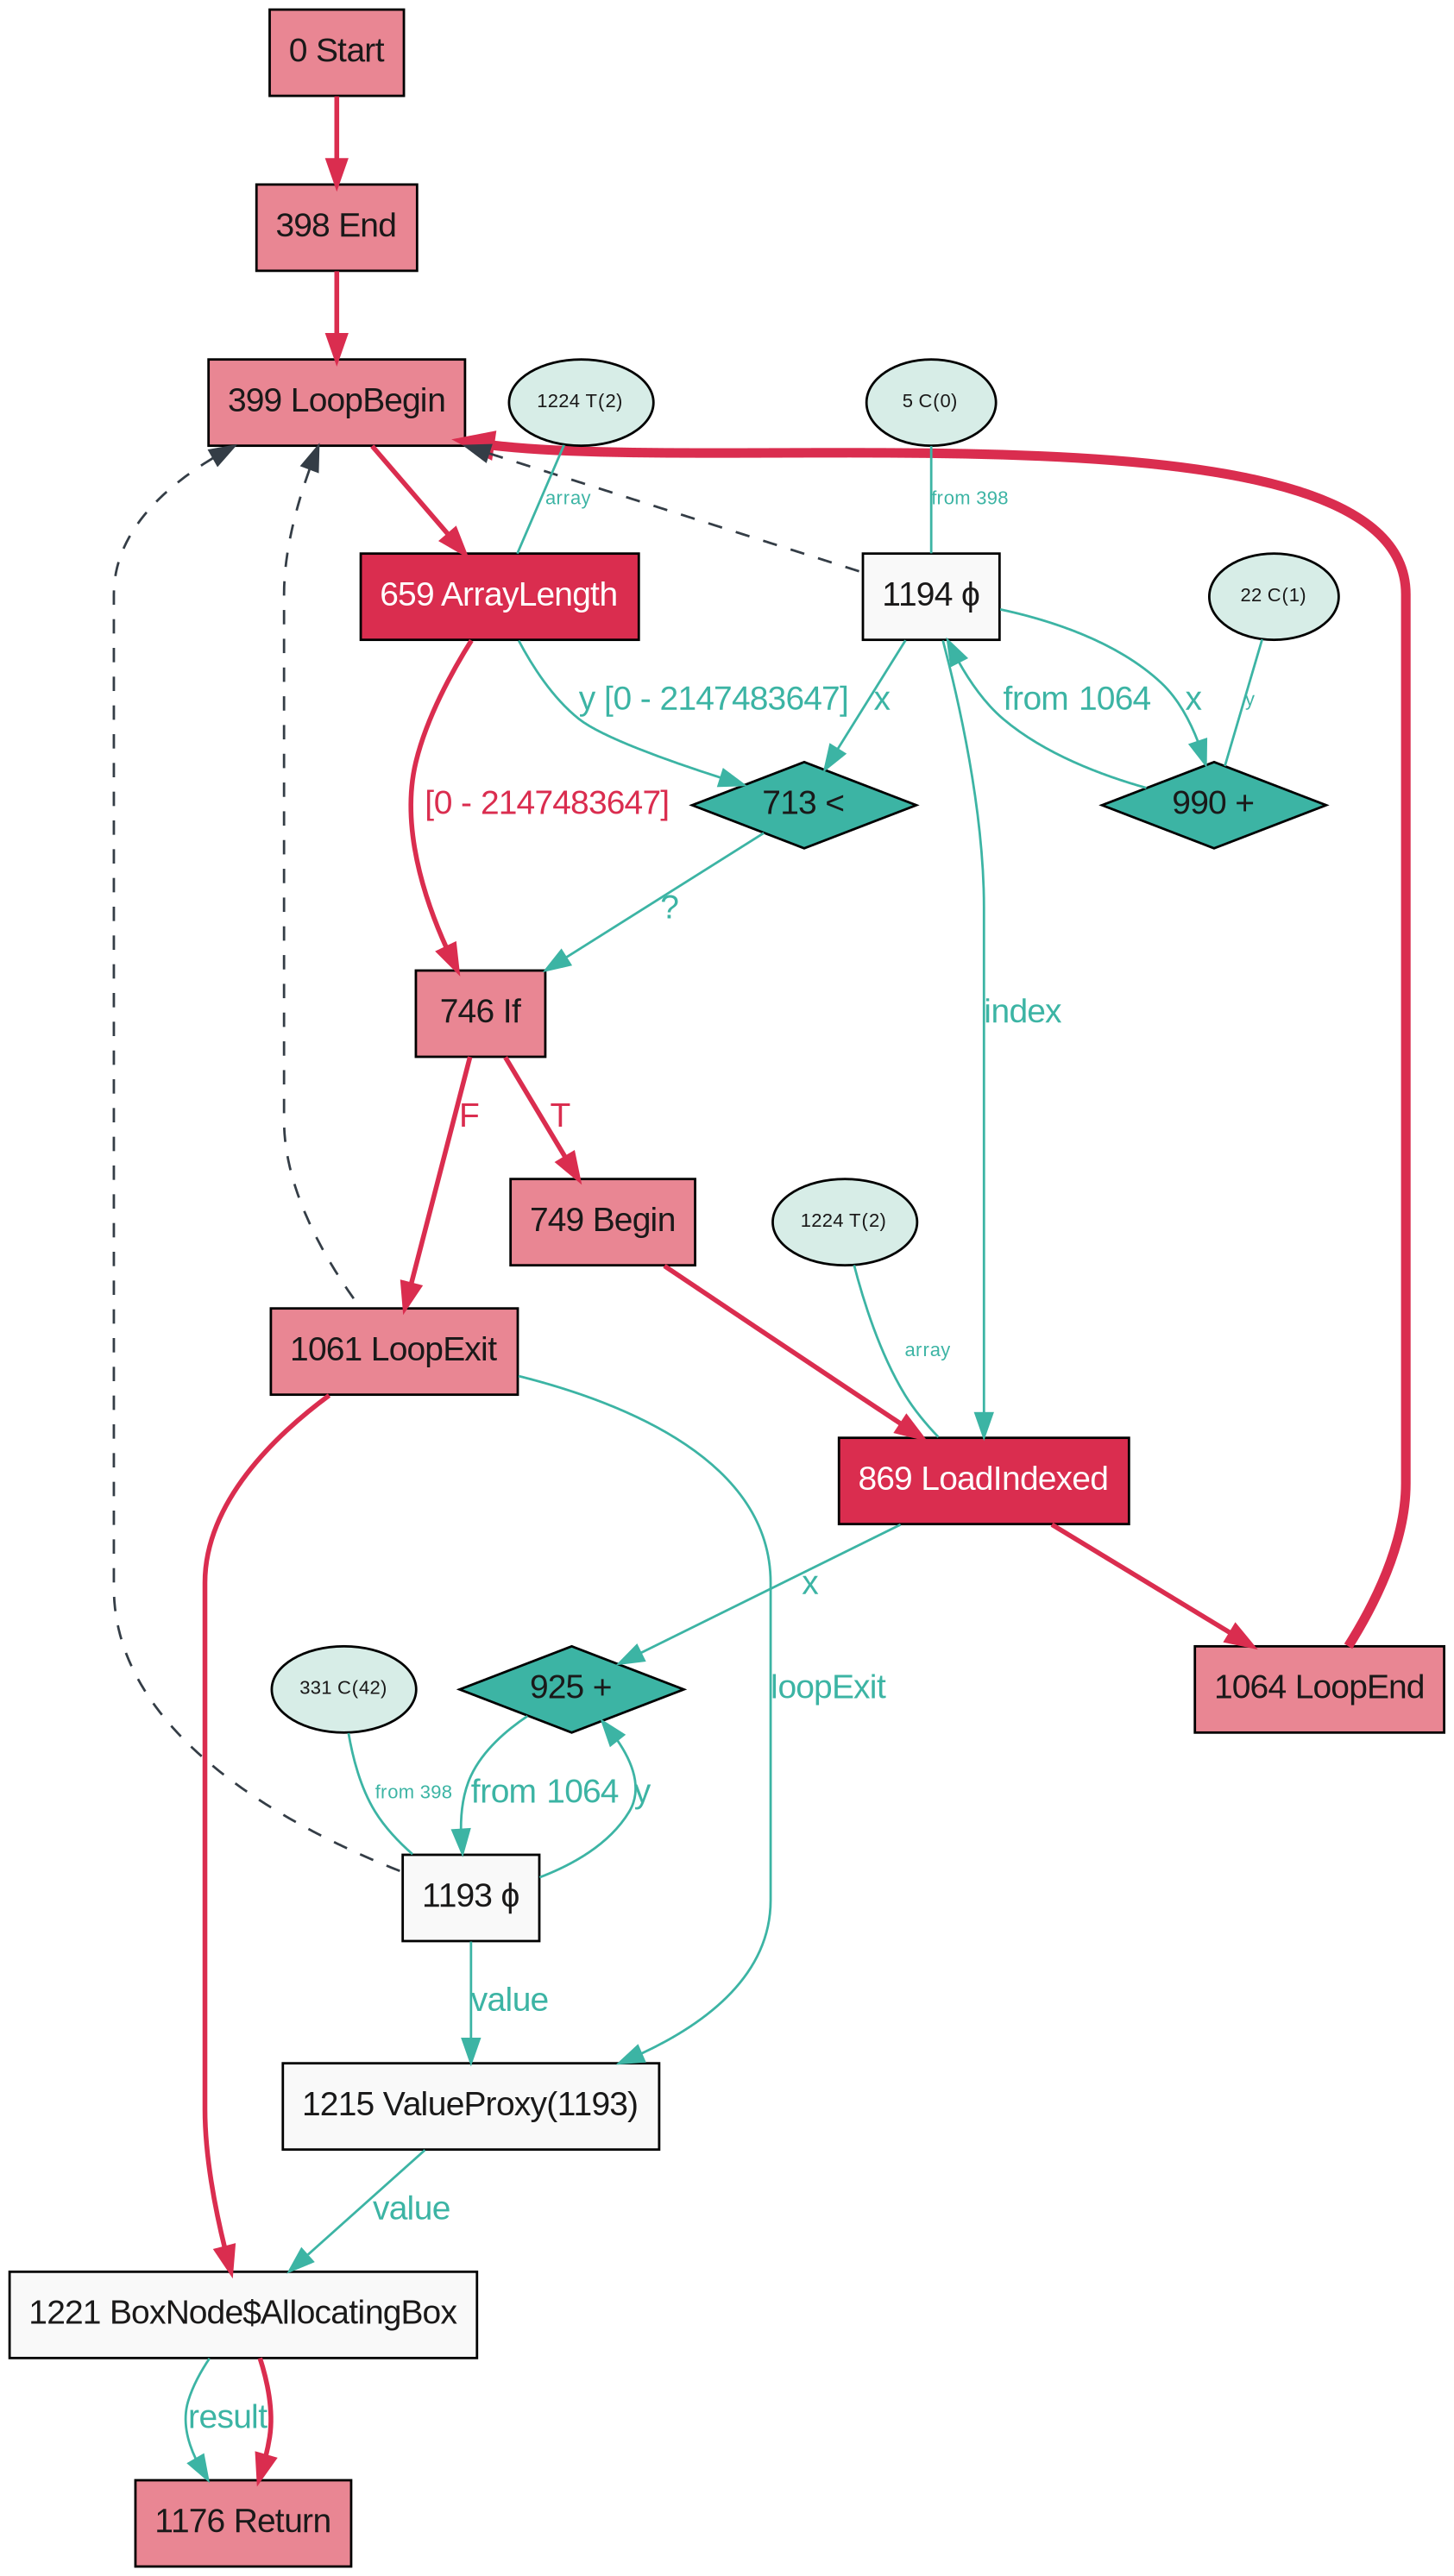
\includegraphics[width=0.5\columnwidth]{figures/checksum:Int:TruffleTier.png}
	\caption{Graal IR graph of specialization \texttt{checksum[Int]} after Truffle tier.}
\end{figure} 